\chapter{Results}

% TODO: Intro

\section{Generation Time}

\begin{figure}[h]
	\centering
	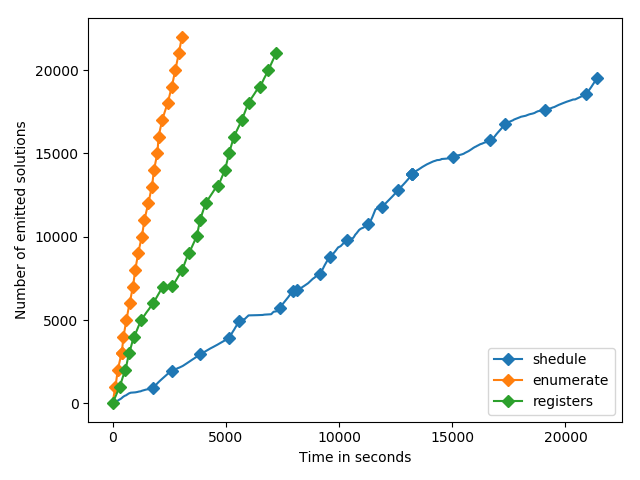
\includegraphics[width=\textwidth,height=0.5\textheight]{results/figures/generator_time}
	\caption{The execution time of the code generator at sampling rate 1000 (i.e 1000000 solutions for every function). Each marker represents the finished generation of a function. The markers are ordered so that the nth marker on every line represents the same function. Total time is annotated as hours and minutes.}
	\label{fig:time}
\end{figure}

The execution times of the constraint solver at sampling rate 1000 are shown in Figure
\ref{fig:time}. Each marker represents the completed generation of a function. I.e for each
marker 1000000 (one million) solutions have been explored. For a few functions fewer than
1000 solutions were found (for a complete breakdown see appendix \ref{appendix:function_names}).

While the total execution time is daunting, it does represent about 23 million solutions
found (but only 23000 emitted). The enumerate strategy is fairly quick; 51 minutes for one
million solutions of every function means that on average, one solution was found every
139ns. The same number for registers and schedule is 343ns and 1095ns respectively. To
mitigate the impact of a long execution time the solutions can be emitted directly when
found.

disUnison does not use the same search heuristics as the base Unison model. The disUnison
search heuristics makes implementation easier at the potential cost of execution time. The
problem with optimizing the branching and search heuristics of the model is that the
performance impact will largely have to be determined empirically. Supposedly, the optimal
search heuristic for the registers strategy would not be the same as the optimal search
heuristic for the schedule strategy.

\section{Cost}

\begin{figure}[h]
	\centering
	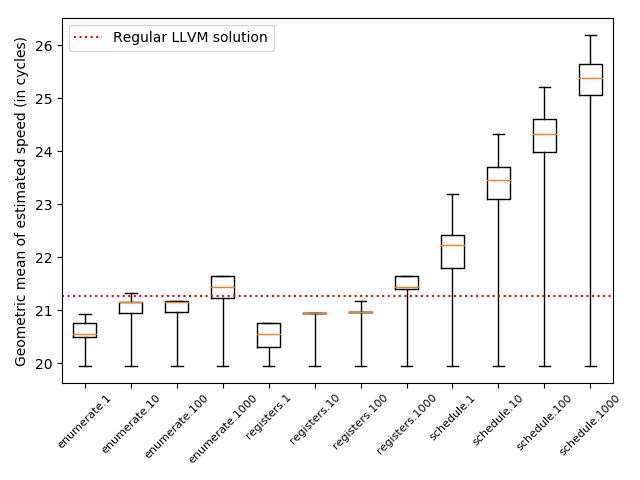
\includegraphics[width=\textwidth,height=0.5\textheight]{results/figures/cost_speed}
	\caption{The cost (speed) distributions for every strategy and sampling rate. The cost of the LLVM solution is included for reference.}
	\label{fig:cost-speed}
\end{figure}

\begin{figure}[h]
	\centering
	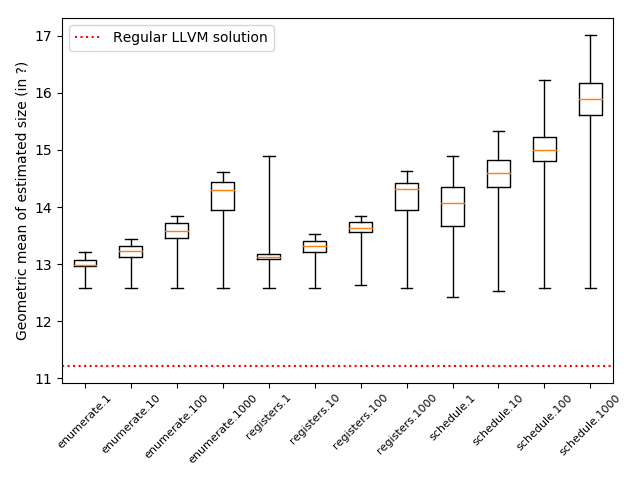
\includegraphics[width=\textwidth,height=0.5\textheight]{results/figures/cost_size}
	\caption{The code size distributions for every strategy and sampling rate. The cost of the LLVM solution is included for reference.}
	\label{fig:cost-size}
\end{figure}

Figure \ref{fig:cost-speed} and Figure \ref{fig:cost-size} shows the distributions of the
estimated cost in cycles and the estimated code size for each strategy and sampling rate
respectively. Both the cost in cycles and the code size for a program version is
calculated as the geometric mean between the cost of the individual functions that make
up a program versions. I.e for every strategy and sampling rate there are 1000 values for
each cost metric, where each value is a geometric mean between the cost values of 23
functions.

All strategies perform better for lower sampling rates both in terms of speed and in terms
of code size. As described in section \ref{sec:sampling_rate}, this is expected. Both the
enumerate and registers strategy performs very well in terms compared to the LLVM solution
in terms of speed. The schedule strategy incurs a slight overhead for the lowest sampling
rate and a significant overhead for the three higher sampling rates.

The fact that no solution has a size lower than the LLVM solution can be explained by
refering to the optimization goal used, which was speed. The code size has not been taken
into account during branching and no attempt has been made to optimize it.

Interesting to note is that all strategies and sampling rates have found a solution with
an equally low speed. This is presumably the very first solution found; When no strategy
related constraints have been posted yet. Thanks to the search heuristic, where lower cost
solutions are explored first, this is also the optimal cost.

\section{Surviving Gadgets}

% Todo: explain y-axis log scale (make all go to 100% as well). Explain why x axis is different

\begin{figure}[htp]
	\centering
	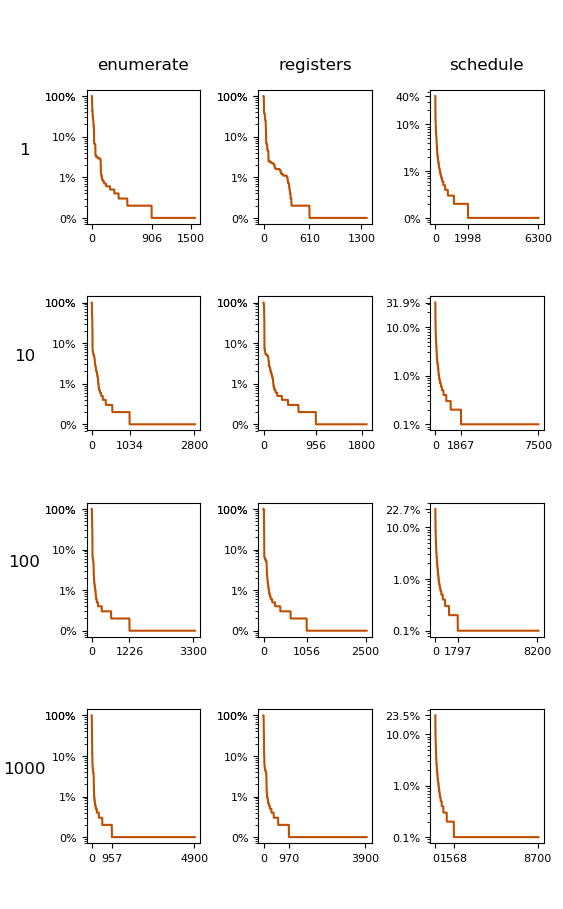
\includegraphics[width=\textwidth,height=\textheight]{results/figures/gadgets}
	\caption{The ratio of occurrence for each gadget broken down by strategy and sampling rate.
Each dot shows the occurrence ratio for one particular gadget. The data is sorted to allow
	for a better overview.}
	\label{fig:gadgets}
\end{figure}

Figure \ref{fig:gadgets} shows the occurrence ratio of each gadget for the different
strategies and sampling rates. The x-axis shows a gadget id and there is no definitive
correlation between the gadgets across strategies and sampling rates. I.e gadget 0 for the
enumerate strategy at sampling rate 1 is not necessarily the same gadget 0 as the registers
strategy at sampling rate 10.

% TODO: Discuss why strategies behave differently with concrete examples
% Perhaps mention that they all find the same first solution and from there the schedule
% strategy makes them differ more. Perhaps mention that for some strategies only 1 solution
% was found (or at least fewer) and explain why. It might make their behaviour clear.

As seen in figure \ref{fig:gadgets}, neither the enumeration nor the registers strategy
were particularly effective at breaking gadgets for any sampling rate. There is a slight
improvement for higher sampling rates but it is not particularly impressive even at
sampling rate 1000. There are still many gadgets that survives across a large percentage of
versions. The schedule strategy, however, performed well with no gadget being present
in even 50\% of all versions for the lowest sampling rate and for sampling rate 1000
about 82\% of gadgets only appear in one version.

% TODO: revise. Super vague
Unfortunately, due to the shortcomings of the experiment this results is not comparable to
the ones presented in other literature. However, it does hint at the potential gadget-
breaking properties of each strategy. Enumerate and registers show decent potential and the
schedule strategy shows great potential but it would have to be verified on a proper
executable for the x86-64 architecture.
